\documentclass[12pt]{article}
\usepackage{authblk}
\usepackage{graphicx}
\usepackage{multirow}
\usepackage{tikz}
\usepackage{caption}
\usepackage{subcaption}
\usepackage{comment}
\usepackage{float}
\usetikzlibrary{positioning}
\usepackage[utf8]{inputenc}
\setlength{\arrayrulewidth}{.5mm}
\setlength{\tabcolsep}{12pt}
\renewcommand{\arraystretch}{.5}
\usepackage[export]{adjustbox}
\graphicspath{{C:/Users/Gauri/Pictures}}
\title{\textbf{Performance  Characterization of String Libraries Implemented with AJIT 64-bit Extensions}}
\author[1]{Gauri Patrikar}
\affil[1]{Project Research Assistant, IITB}
\begin{document}


\maketitle
\begin{abstract}

We have developed string libraries using the SPARC V8 assembly with the newly added extensions to the AJIT processor. These instructions were designed to handle 64 bits at once and aid in enhancing the performance. 


The libraries have been written in assembly instead of C as it is more chanllenging to develop a compiler.


The performance for implemented string functions is characterized and improvement in performance is noted for all. 
The libraries were compared with the existing uclibc C string libraries.
 \end{abstract}

\section{Introduction}
\subsection{64 bit extensions}
The AJIT processor is based on the 32 bit SPARC V8 ISA.  New assembly instructions that perform 64 bit operations have been added to enhance the performance
Some  examples of the 64 bit extensions that were used were-
\begin{itemize}
    \item zbytedpos - gives an 8 bit output corresponding to a 64 bit input. It checks if any byte in the input is zero and sets the corresponding output bit to 1, else bit is set to 0.
    \item addd - performs 64 bit addition, result is also 64 bit.
    \item subdcc - performs a 64 bit subtraction while setting condition codes.
    \item ord - performs a 64 bit or, result is also 64 bit.
    \item srld  - performs a maximum of 64 bit logical right shift.
\end{itemize}

These instructions are performed in a single clock cycle and  help reduce number of operations, hence make string manipulation much faster.\newline
Strings terminate with a null byte. Hence, finding the zeroth byte is important. Using the zbytedpos instruction, we can find the null byte in a 64 bit number in one instruction itself. In case of other instructions also, operations are performed two at once, for eg., increment two memory locations at once. This decreases the number of instructions required. 

\subsection{Sparc ABI}
The programs have been written in assembly, simply because generating a compiler was a more complex task. 

These libraries can be called using a C program.
These programs are based on the SPARC ABI protocol. It is a calling convention used when an assembly program needs to be called using a C program.  It gives the protocol for argument passing, writing the prologue and epilogue of the assembly functions and so on. This ensures that the process of shifting between the C and the assembly programs is seamless. 

\subsection{Restrictions}

One restriction that holds in all these functions is that the addresses of the two strings need to be doubleword aligned. This is checked before starting each program.

In case of the strcat function, the termination of destination string should also be doubleword aligned.

If they are not aligned the code will exit without doing anything.

\subsection{Functions and comparisons}
The following functions are being implemented here -
\begin{enumerate}
    \item strcpy
    \item strncpy
    \item strcmp
    \item strcasecmp
    \item strcat
\end{enumerate}
.
We are comparing these new libraries with the uclibc string library. Both of them are compiled to the SPARC V8. An improvement of about 40\% to 90\% was observed in the various functions 


\subsection{Accessing Libraries}

To access these libraries, add include "a64string.h", which contains the definitions for all of the functions. Further details for each function are given below.\newline
The functions can be called using  c program, as you would call any other string library, adding 'a64' to the name of the function, eg. strcmp funciton can be called by a64strcmp. All the inputs are exactly the same as the existing libraries, as is given in detail below.


Each function is described in the following sections. Its inputs and expected outputs are described below.


\section{a64strcpy}
The function copies the string pointed to by src, including the terminating null byte, to the buffer pointed to by dest. You can call it using -
\begin{verbatim}
char a64strcpy(char *dest, char *src);
\end{verbatim}
The strings may not overlap, and the destination string dest must be large enough to receive the copy.

It returns the pointer to the destination string.


\subsection{Program Flow}

Following is a brief description of the how the program works. We use two instructions from the new extensions- zbytedpos, srld and addd. 

\begin{enumerate}
    \item Check memory alignment, has to be 64 bit aligned.
    \item If aligned, operate in 64 bit mode, else return.
    \item If aligned, load doubleword from memory.
    \item Check for null byte using the new zbytedpos instruction. Compare with zero to see if null byte exists.
    \item If no null byte, increment both memory locations using the new addd instruction, and perform a double word store.
    \item Repeat this process till null byte found.
    \item Check which byte is null, by shifting each byte and comparing .
    \item if it is not null, increment memory and store byte,
    \item continue till null byte found and return.
\end{enumerate}

\section{a64strncpy}
First n bytes of src is copied to dest. You can call it using -
\begin{verbatim}
    astrncpy (char *dest, char*src, size_t n)
\end{verbatim}

Even if no null byte found in these n bytes and if length of dest is smaller than src, dest will not be not null terminated.

If there a null byte among the first N bytes, the rest of the length of dest is written with null bytes.


It returns a pointer to the destination string.


\subsection{Program Flow}

Following is a brief description of the how the program works. We use two instructions from the new extensions- zbytedpos,srld and addd. 


\begin{enumerate}
   \item Check memory alignment, has to be 64 bit aligned.
    \item If aligned, operate in 64 bit mode, else return.
    \item If aligned, load doubleword from memory.
    \item Decrement counter and check if n is less than zero.
    \item If greater than zero, check for null byte using the new zbytedpos instruction. Compare with zero to see if null byte exists.
    \item If no null byte, increment both memory locations using the new addd instruction, and perform a double word store.
    \item Repeat this until either n is less than or equal to zero or null byte is found.
    \item If n is less than zero, icremenr it and start loading and string bytewise till n is zero.
    \item end program at n = 0.
 
\end{enumerate}

\section{a64strcmp}
The function  compares  the two strings s1 and s2. You can call it using -
\begin{verbatim}
  char astrcmp (char* s1, char *s2)  
\end{verbatim}
It returns the difference between the two strings(s1-s2).



\subsection{Program Flow}

Following is a brief description of the how the program works. We use three instructions from the new extensions- zbytedpos, subdcc and addd. 


\begin{enumerate}
   \item Check memory alignment, has to be 64 bit aligned.
    \item If aligned, operate in 64 bit mode, else bytewise.
    \item If aligned, load doubleword from memory for both strings.
    \item Compare both doublewords for equivalence.
    \item Check for null byte using the new zbytedpos instruction for both the strings Compare with zero to see if null byte exists.
    \item If no null byte, increment both memory locations using the new addd instruction.
    \item Repeat this process till either null byte is found or the two strings are different.
    \item If it is equal, and null byte is found, we can say the strings are equal.
    \item If unequal, go bytewise to check exact byte where it differs.
    \item return when the different byte is found.
\end{enumerate}

\section{a64strcasecmp}
The astrcasecmp function is similar to astrcmp, except it compares ignoring the case of the string. You can call it using -

\begin{verbatim}
   astrcasecmp (char *s1, char *s2)  
\end{verbatim}

It compares the two strings s1 and s2 ignorng the case of the byte. For eg., the byte 'a' and 'A' should be considered equivalent. and It returns the difference between the two strings (s1-s2)



\subsection{Program Flow}

Following is a brief description of the how the program works. We use three instructions from the new extensions- zbytedpos, subdcc and addd. 

\begin{enumerate}
   \item Check memory alignment, has to be 64 bit aligned.
    \item If aligned, operate in 64 bit mode, else return.
    \item If aligned, load doubleword from memory for both strings.
    \item Make them lovercase by making 6th bit of each byte as '1'.
    \item Check if strings are equal.
    \item Check for null byte using the new zbytedpos instruction for both the strings Compare with zero to see if null byte exists.
    \item If no null byte, increment both memory locations.
    using the new addd instruction.
    \item Repeat this process till either null byte is found, or the two strings are different.
    \item If equal, but null byte, then the two strings are equal.
    \item If unequal, check which byte is unequal.
    \item return when different byte is found.
    
\end{enumerate}

\section{a64strcat}
The function copies the string pointed to by src, including the terminating null byte, to the end of the dest string. You can call it using -
\begin{verbatim}
char astrcat(char *dest, char *src);
\end{verbatim}


Here, the dest string must also terminate at 64 bit aligned memory boundary. This is to ensure that the source can perform doubleword stores to the dest string.
The strings may not overlap, and the destination string dest must be large enough to receive the copy.

It returns the pointer to the destination string.

\subsection{Program Flow}

Following is a brief description of the how the program works. We use two instructions from the new extensions- zbytedpos,srld and addd. 


\begin{enumerate}
    \item Check memory alignment, has to be 64 bit aligned.
    \item If aligned, operate in 64 bit mode, else return.
    \item Increment memory till null of dest string is found. This is the memory that the src string will copy to.
    \item If aligned, load doubleword from memory.
    \item Check for null byte using the new zbytedpos instruction. Compare with zero to see if null byte exists.
    \item If no null byte, increment both memory locations using the new addd instruction, and perform a double word store.
    \item Repeat this process till null byte found.
    \item Check which byte is null, by shifting each byte and comparing .
    \item if it is not null, increment memory and store byte,
    \item continue till null byte found and return.
\end{enumerate}

\section{Performance comparison}
As we can see from the figure, improvement of minimum of 40\% and a maximum of upto 90\% is observed.


This reduce in instructions is mainly due to the fact that about only half the number of iterations were required in the main loops (where maximum time is spent by the function), as we could use 64 bit operations.

\begin{figure}[H]
     \centering
     \begin{subfigure}[b]{0.4\textwidth}
         \centering
         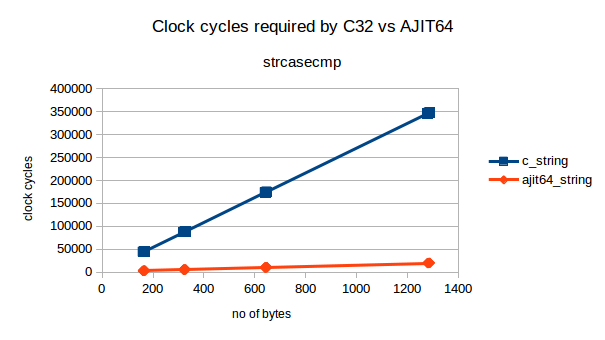
\includegraphics[width=\textwidth]{strcasecmp.png}
         \caption{strcasecmp}
     \end{subfigure}
     \hfill
     \begin{subfigure}[b]{0.4\textwidth}
         \centering
         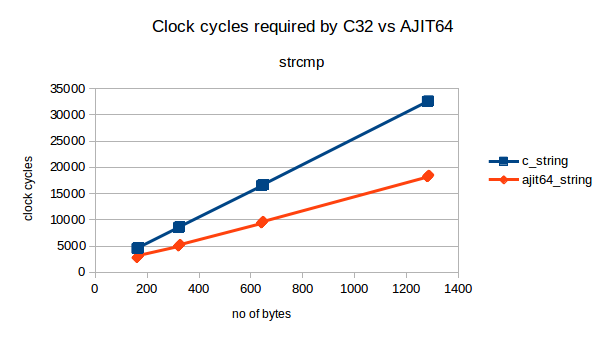
\includegraphics[width=\textwidth]{strcmp.png}
         \caption{strcmp}
         \end{subfigure}
     \hfill
     \begin{subfigure}[b]{0.4\textwidth}
         \centering
         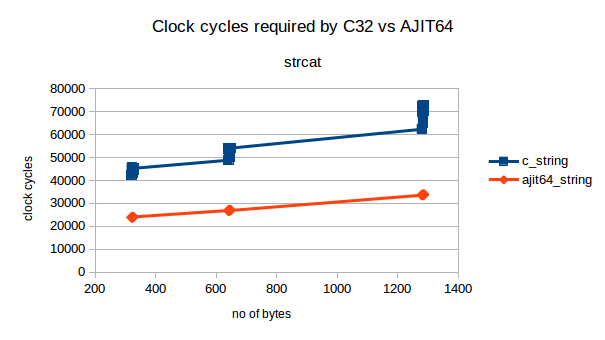
\includegraphics[width=\textwidth]{strcat.png}
         \caption{strcat}
     \end{subfigure}
       \hfill
     \begin{subfigure}[b]{0.4\textwidth}
         \centering
         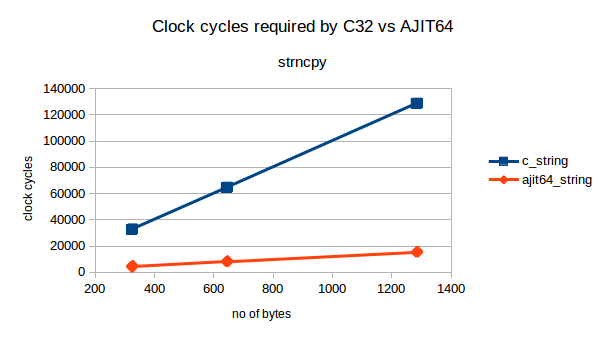
\includegraphics[width=\textwidth]{strncpy.png}
         \caption{strncpy}
         \end{subfigure}
       \hfill
     \begin{subfigure}[b]{0.4\textwidth}
         \centering
         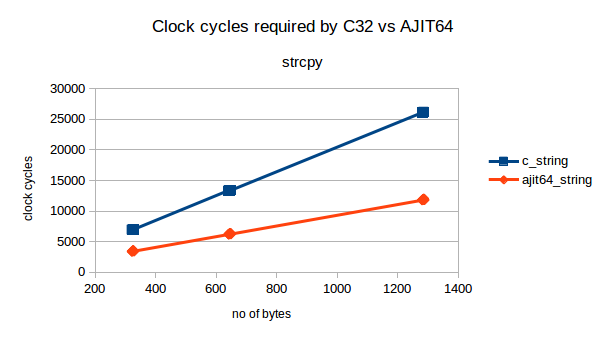
\includegraphics[width=\textwidth]{strcpy.png}
         \caption{strcpy}
     \end{subfigure}
        \caption{String functions}
        \label{fig:three graphs}
\end{figure}

\newpage

\section{Conclusion}
An implementation of the string libraries using 64 bit instructions in assembly was discussed. The performance was compared to that of the existing uclibc C string libraries.
\newline
Performance improvement was observed in all cases. In case of strncpy and strcasecmp functions, a 
significant improvement of 80\%-92\% was observed.
\newline

We conclude that these libraries can be used for performance enhancement.

 \end{document}
